\begin{figure}[!htbp]
    \centering
    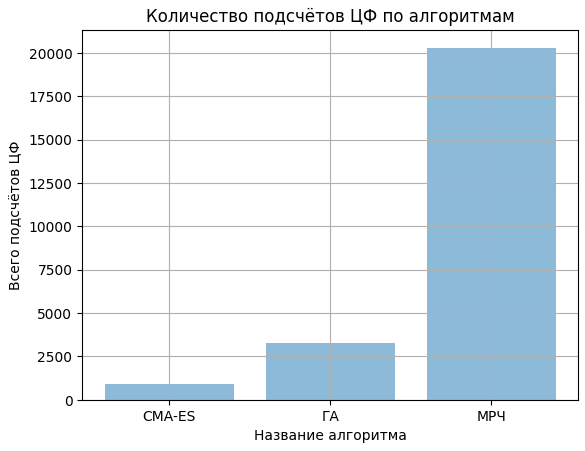
\includegraphics[height=0.38\textheight,valign=t]{my_folder/images//evalsall.png}
    
\captionsetup{justification=centering} %центрировать
\caption{Гистограмма, отображающая $N_f$} \label{fig:hist-wd}
\end{figure}

\begin{figure}[!htbp]
    \centering
    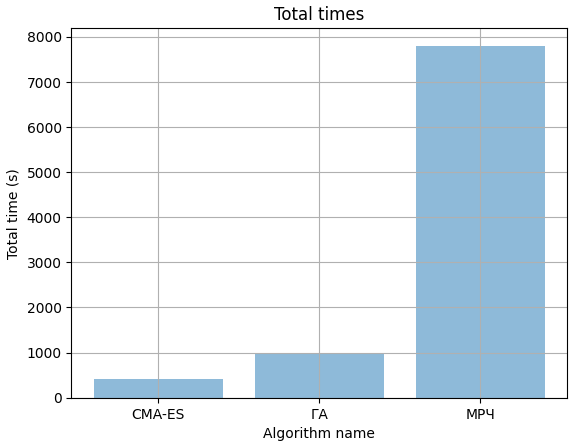
\includegraphics[height=0.38\textheight,valign=t]{my_folder/images//total-times.png}
    
\captionsetup{justification=centering} %центрировать
\caption{Гистограмма, отображающая  $T_{\text{общ}}$} \label{fig:hist-times-wd}
\end{figure}